\documentclass{book}
%\standalonetrue
\usepackage{import}
\subimport{../}{preamble}
\begin{document}

\section{Axial Scanning of Tip Dimers}
\label{sec:tip_scanning}

\begin{figure}[h]
\centering
\fcapside[\FBwidth]
{\subimport{./figures/}{simple_optics_dimer_layout.tex}}
{\caption[Experiment configuration for axial tip scanning]{\textbf{Experiment configuration for axial tip scanning.} The laser is centered on the aligned tip dimer for gap spectroscopy. The soft cantilever approaches the stationary, stiff cantilever at a rate $dz$ \si{\nano\metre\per\second}. A bias is applied across the tip junction and the current through the gap is measured. The soft cantilever faces the AFM module for force measurement via cantilever deflection.}
\label{fig:simple_optics_dimer_layout}}
\end{figure}

% Optics
Once two tips are aligned into an opposing dimer configuration their separation-dependent properties, such as plasmonic interaction, can be dynamically explored. To do this effectively the optical and electronic properties are simultaneously measured along with the applied force. These are measured by holding one of the tips stationary in the collection volume, which acts as the optical probe, while the other tip approaches at a rate of 0.1--\SI{1}{\nano\metre\per\second}. The probe tip is typically positioned moreso in the collection volume compared to the approaching tip since it is aligned with the beam to give good signal prior to alignment between tips. The approaching tip perturbs the near-field and therefore interacts with the probe tip. Gap-dependent plasmon coupling scatters into the objective collection aperture via outcoupling with plasmonic antenna modes in the probe tip.
% Electronics
The electronic properties are probed by driving with a d.c. applied bias and measuring the current through the dimer to determine the conductivity of the junction. The bias is usually set to \SI{50}{mV} to achieve good signal to noise in both the low-bandwidth and high-bandwidth conductance measurements and to prevent noise from setting off the high-bandwidth trigger.
% Force
The applied force is measured using optical detection of the cantilever deflection in the AFM module. The microscope configuration used for such experiments is shown in \figurename~\ref{fig:simple_optics_dimer_layout}. Using this combination of measurements allows for a proper understanding of nanoscale gap behaviour.

\begin{figure}[h]
\centering
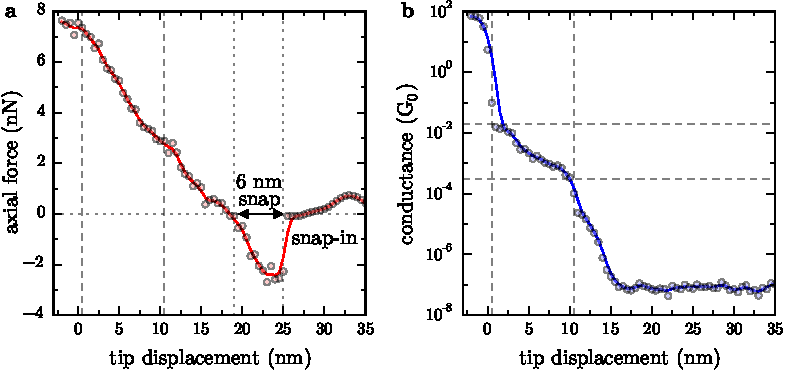
\includegraphics{figures/tip_scanning_properties}
\caption[Axial force and conductance measurements of a sharp Au tip dimer approaching into contact]{\textbf{Axial force and conductance measurements of a sharp Au tip dimer approaching into contact.} The characteristic AFM snap-in effect is seen as a discontinuous jump before the linear application of force regime. The tip apices snap together, reducing the separation to on the order of \SI{1}{nm}, leading to the onset of quantum tunnelling upon further decreasing the gap separation.}
\label{fig:tip_scan_props}
\end{figure}

% Snap-in
Since the experiments are carried out in ambient conditions the surface of the tips will always be coated in a thin film of water or nanobubbles. Even in a nitrogen environment water is still present, although the thickness is reduced. When two coated surfaces come into close proximity a water meniscus forms between them leading to strong capillary forces, hence when the separation between the two tips reduces past a certain point they are quickly pulled together \cite{holmberg2013}. This is known in AFM literature as the "snap-in" or "snap-into-contact" and occurs on separations $\sim10--\SI{30}{nm}$ \cite{holmberg2003, song2014}.

The snap-in is clearly seen in axial force measurements as a discontinuous jump towards the stationary tip (\figurename~\ref{fig:tip_scan_props}a). To prevent snap-in the water meniscus has to be removed, which is usually achieved through liquid immersion AFM \cite{}, though can be achieved using plasma treatment to remove hydrophobic contamination \cite{song2014}. To our advantage, however, the presence of a meniscus in the gap prevents immediate electrical contact between tips and holds the gap at  $\sim\SI{1}{nm}$ until further force is applied. This effectively splits a scan into three regimes, one in which the piezo distance corresponds directly to a separation decrease between tips, one in which the piezo distance corresponds to increasing the applied force on the meniscus (soft interaction) and finally one in which the force is applied directly to the opposite tip (hard-wall contact). The existence of the soft interaction regime allows for sub-nm gaps to be studied with some degree of control since only a fraction of the applied probe displacement corresponds to the displacement of the apex. Instead, the meniscus is loaded with the applied force leading to a linear reverse deflection observed in AFM force measurements as the tip progresses forwards. This can be seen in \figurename~\ref{fig:tip_scan_props} where \SI{15}{nm} of cantilever displacement moves the apex $\sim\SI{0.8}{nm}$ (deduced from electron tunnelling measurements). The remaining \SI{14.2}{nm} loads the gap with an applied force of \SI{8}{nN}, proportional to the tips spring constant.

Electron tunnelling is the dominant charge transfer mechanism, occurring prior to geometrical (conductive, $G<1\G0$) contact. It is often approximated using the Simmon's equation \cite{tan2014},
\begin{equation} J=J_0e^{-\beta d}, \end{equation}
where $d$ is the separation, $J$ is the current density, $J_0$ is the saturation current density at $d=0$ and,
\begin{equation} \beta = \sqrt{\frac{2m\varphi}{\hbar^2}}, \end{equation}
is the decay rate consisting of the barrier work function $\varphi$.

% Charge transfer
Upon reducing the gap to below \SI{1}{nm} electron tunnelling becomes detectable. The current due to tunnelling follows an exponential growth $I = e^{kd}$ therefore for every \SI{1}{\angstrom} (\SI{0.1}{nm}) away from geometrical (conductive) contact the transmission drops by a factor of 10 \cite{}. Though the absolute value of the conductance for a given separation depends on the gap morphology the relative exponential conductance drop from geometrical contact still approximately holds for $d>\SI{2}{\angstrom} $\cite{esteban2014classical}. This makes electron tunnelling a useful method for determining the gap size to within \SI{0.1}{nm}, as is done in STM, though the technique is limited to sub-nm separations. Once the separation is greater than \SI{1}{nm} the conductance drops from $1\G0$ at conductive contact to $10^{-10}\G0$ and the corresponding current becomes difficult to measure without significantly raising the d.c. bias. Use of a large bias of \SI{50}{mV} still means a current on the order of \SI{0.1}{fA}\footnote{$10^{-16}\si{A}$}, which remains below the noise level achievable in the current setup. Increasing the bias also increasing the electrostatic forces pulling the tips together, therefore decreasing the effective gap resolution in the sub-nm regime.
% effect of water in the gap on tunnelling calibration? effect of finite large surface?

\figurename~\ref{fig:tip_scan_props}b shows a typical conductance trace on approach. Once the separation decreases below \SI{1}{nm} the conductance quickly increases from \num{e-8} to around $10^{-3}\G0$ as the tips transition through the soft interaction regime, at which point the rate of increase slows. {\color{red}This is thought to be caused by displacing the water layer until only a \SI{3}{\angstrom} gap film remains, which may or may not be more solid than the original water film.} A larger force is required to push through this layer and into conductive contact. Once the gap reduces below \SI{2}{\angstrom} there is usually a sharp increase in the current as it transitions into full conductive contact, ranging between $1\G0$ and $200\G0$.

%The use of tunnelling currents as a distance measure also means that the gap size can potentially be stabilised in the sub-nm regime by using a feedback loop, thus operating more like a traditional STM.

Both the force and the conductance provide significant insight into the structure and dynamics of nanoscale gaps and become especially useful when correlating spectral changes that depend sensitively on the gap morphology and dielectric medium. From this information more accurate physical models can be developed to further understand the sub-nm plasmonics regime.

\end{document}